\documentclass{scu-thesis}
\usepackage[pass,letterpaper]{geometry}
% \usepackage{graphicx}	% for including graphics
% \usepackage{amsmath}	% for advanced typesetting of mathematics
\usepackage{txfonts}	% for using the Times-Roman font
% \usepackage{natbib}	% for better citation styles
\usepackage{parskip}



% These must be set first ... the rest of the thesis commands rely on them.

\author{Melissa Bica}
\author{Elizabeth Donahue}
\title{Text To Learn: A Digital Training System for Global Social Enterprises}
\department{Department of Computer Engineering}
\degree{Bachelor of Science in Computer Science and Engineering}


% Only bachelor's theses should have multiple authors and/or be from
% multiple departments.  Signatures required:
%
% Bachelor's theses: advisor(s), department chair(s)
% Master's theses: advisor, reader, department chair
% Doctoral theses: doctoral committee (including advisor), department chair

\begin{document}
\frontmatter
\signature{Thesis Advisor}
\signature{Department Chair}

\maketitle
\begin{abstract}
Text to Learn is a training tool made with Social Enterprises in mind that uses SMS to distribute training materials and to test users on their learning. Our goal is to give social enterprises a way to train employees and customers digitally and remotely. We will create an online dashboard, using RapidSMS and a cloud storage service, for social enterprises to upload and send training materials, manage users, and create SMS-based quizzes to assess users’ progress.
\end{abstract}

\include{acknowledgements}

\tableofcontents
\listoffigures
\listoftables

\mainmatter
\chapter{Introduction}

\section{Background}

Social enterprises are rising in prevalence in developing countries to help address issues related to social, economic, environmental, and other issues that these countries face. We worked with two different social enterprises in Nepal and India, respectively, and saw the life-changing work they do for extremely disadvantaged people. However, we also encountered some of the problems that these types of organizations face, especially concerning training of employees. Many factors contribute to the difficulty social enterprises have in providing proper and effective training for their employees, including fewer resources relative to other types of organizations and logistical barriers inherent to working in developing countries. Employee training is vital for social enterprises to succeed in both their social missions and business goals, and cannot be taken for granted in the context of the developing world.

Social enterprises take on various approaches to training their employees, but most of these approaches do not overcome the barriers described above. Anudip, the organization Melissa worked with in India, holds annual Training of Trainers events, where hundreds of trainers gather and receive formal lessons on how to teach new employees either English/workplace readiness or information technology (IT) skills. While this event is great for uniting all of the Anudip trainers and sharing ideas, it is not necessarily the most effective way to train employees. The training was impersonal due to such a large number of people, and many of the employees seemed unfamiliar with the material that they were supposed to teach to others. 

Anudip also has informal training in each of its centers, which typically is conducted by having the trainer working at a computer and explaining the material to a group of employees crowded around her. Anudip, like many social enterprises, does not have the resources for designated classrooms, so training happens in the main workspace alongside other working employees. Additionally, this informal training, while very personal, can be fast-paced and overcrowded, making it hard for employees to learn the material effectively. Our senior design project addresses these difficulties social enterprises face in trying to train employees.

Our solution to this issue of training in social enterprises is to use mobile phones, which are becoming increasingly popular in developing countries. We have developed Text to Learn as a system for trainers within social enterprises to upload digital training materials to a common repository. This information can then be sent as SMS text messages to the mobile phones of employees who are registered by the trainers. Text to Learn is interactive with the addition of quizzes created by the trainers. Registered employees can respond to these quizzes via SMS. 

This product addresses the issue of lack of resources by utilizing a resource that nearly all people, even in developing countries, already have--the mobile phone. More specifically, we have developed the system to be used on feature phones, which are less advanced than smartphones and much more common in the developing world. Furthermore, this product overcomes the logistical barriers many social enterprises face by allowing training and learning of materials to be done on employees’ own time, at their own pace, and in their own space. Employees will have full access to training materials as they will be stored on their personal feature phones. They will also not be limited to training only at work where computers are available, but can learn from the materials on their phones at home as well. 

Ultimately, Text to Learn is an affordable, adaptable, accessible, and appropriate solution for social enterprises to provide vital training to their customers and employees and continue producing social benefit for the developing world.


\section{Project Overview}
Our system is a website interface for social enterprises to upload and send training materials and quizzes, which are sent as SMS messages to trainees’ mobile phones. Through the website, trainers are also able to manage users, keep track of all messages sent and received, and monitor users' progress on training and quizzes. Text to Learn could be used in addition to or in place of other traditional training methods.

\chapter{System Requirements}


\section{Requirements}
From discussions with a social entrepreneur, CEO of Anudip Dr. Radha Basu, and from our own experiences working with social enterprises, we have compiled the following list of requirements for this project: \\[-0.7\baselineskip]

\underline{Functional}\\
\textit{Critical}
\begin{itemize}
\item Distributors are able to make training materials available to trainees digitally.
\item Distributors are able to test trainees’ knowledge of training materials.
\item Distributors are able to view results of quizzes.
\item Distributors are able to enable/disable quizzes.
\item Distributors are able to register/unregister trainees for use of system.
\item Trainees are able to access training materials.
\item Trainees are able to receive training materials in small pieces.
\end{itemize}

\textit{Recommended}
\begin{itemize}
\item Distributors are able to send notifications when new training materials are added.
\item Trainees are able to automatically receive results from quiz.
\item Trainees are able to view their progress.
\item Trainees are able to access notifications/training materials multiple times.
\end{itemize}

\textit{Suggested}
\begin{itemize}
\item Distributors are able to set a time limit on the completion of quizzes.\\[-0.5\baselineskip]
\end{itemize}

\underline{Non-Functional}\\*
\textit{Critical}
\begin{itemize}
\item Compatible with basic/feature phones.
\item Easy to read.
\item Low distribution costs for social enterprises.
\item Portable to different web and mobile platforms.
\item Maintainable.
\end{itemize}

\textit{Recommended}
\begin{itemize}
\item Scalable for more users.
\end{itemize}

\textit{Suggested}
\begin{itemize}
\item Open source, extensible.
\item Support for multiple languages.
\end{itemize}

\section{Use Cases}
For our implementation, we have come up with several key use cases for the two types of users of our system: distributors (or trainers) and trainees. The following figures visually describe the main functions for each type of user. The primary use cases are also described in greater detail below.

\underline{Case 1 - Upload Materials}\\*
\textit{Actor:} Distributor\\*
\textit{Goal:} Materials with related quiz are ready to distribute.\\*
\textit{Preconditions:} Have materials in a plaintext format, be a registered user, and internet connection.\\*
\textit{Postconditions:} Materials are uploaded and a quiz is created.\\*
\textit{Scenario:}
\begin{enumerate}
	\item{Navigate to the “Add New Materials” page.}
	\item{Enter text of training materials into the box.}
	\item{Write in the questions answers in the appropriate boxes.}
	\item{Hit Submit.}
\end{enumerate}
\textit{Exceptions:}
\begin{enumerate}
	\item{Text is too long to process.}
	\item{Something on the site is broken.}\\
\end{enumerate}

\underline{Case 2 - Add Users}\\*
\textit{Actor:} Distributor\\*
\textit{Goal:} Grant access to training materials to their employees.\\*
\textit{Preconditions:} Be a registered user, know the phone-number the employee will be using.\\*
\textit{Postconditions:} A registered user can download training materials.\\*
\textit{Scenario:}
\begin{enumerate}
	\item{Navigate to the “Manage Users” page.}
	\item{Select “Add New” by the list of users.}
	\item{Enter the new User’s mobile number and additional information such as name and trainee group.}
	\item{Hit submit to store the number and send a verification text to the trainee.}
\end{enumerate}
\textit{Exceptions:}
\begin{enumerate}
	\item{Incorrect mobile number.}\\
\end{enumerate}

\underline{Case 3 - Manage/Edit Training Materials}\\*
\textit{Actor:} Distributor\\*
\textit{Goal:} Ability to view and edit all uploaded training materials, quizzes, and related SMS messages.\\*
\textit{Preconditions:} Be a registered user, have previously uploaded training materials, and internet connection.\\*
\textit{Postconditions:} Training materials can be edited.\\*
\textit{Scenario:}
\begin{enumerate}
	\item{Navigate to the content dashboard.}
	\item{To view or edit existing training materials, click on “Manage” within the Training Materials Panel.}
	\item{View the list of all training materials (in plain text), all SMS messages sent, and all quizzes sent.}
	\item{Select “Edit” to edit these existing materials.}
	\item{To add a new training material, click on “Add new” within the Training Materials Panel.}
	\item{Follow use case above for Upload Materials.}
\end{enumerate}
\textit{Exceptions:}
\begin{enumerate}
	\item{Cannot edit texts that have already been sent; must send new version.}\\
\end{enumerate}

\underline{Case 4 - Take Quiz}\\*
\textit{Actor:} Trainee\\*
\textit{Goal:} Respond to quizzes based on specific training materials.\\*
\textit{Preconditions:} Trainee is registered by trainer and has received and completed reading training materials on phone.\\*
\textit{Postconditions:} Trainee can submit responses to quiz.\\*
\textit{Scenario:}
\begin{enumerate}
	\item{Trainee responds to prompt to begin quiz.}
	\item{Receives quiz on phone as SMS message.}
	\item{Responds to questions by texting back his or her answer.}
	\item{Quiz results are sent back to webpage to be parsed and stored in cloud.}
\end{enumerate}
\textit{Exceptions:}
\begin{enumerate}
	\item{Quiz is not available.}
\end{enumerate}
\chapter{Design and Implementation}

\section{Trainer Interface: The Website}
The following are screenshots of the website we designed and built for the trainers. These five images show the main pages of our website: Home, Add a User, Training Materials, Assign Training Material, and Message Log. The goal is a clean, simple interface that is intuitive and functional. Additional screenshots from the website are included in the Appendices.

\begin{figure}[H]
	\centering
	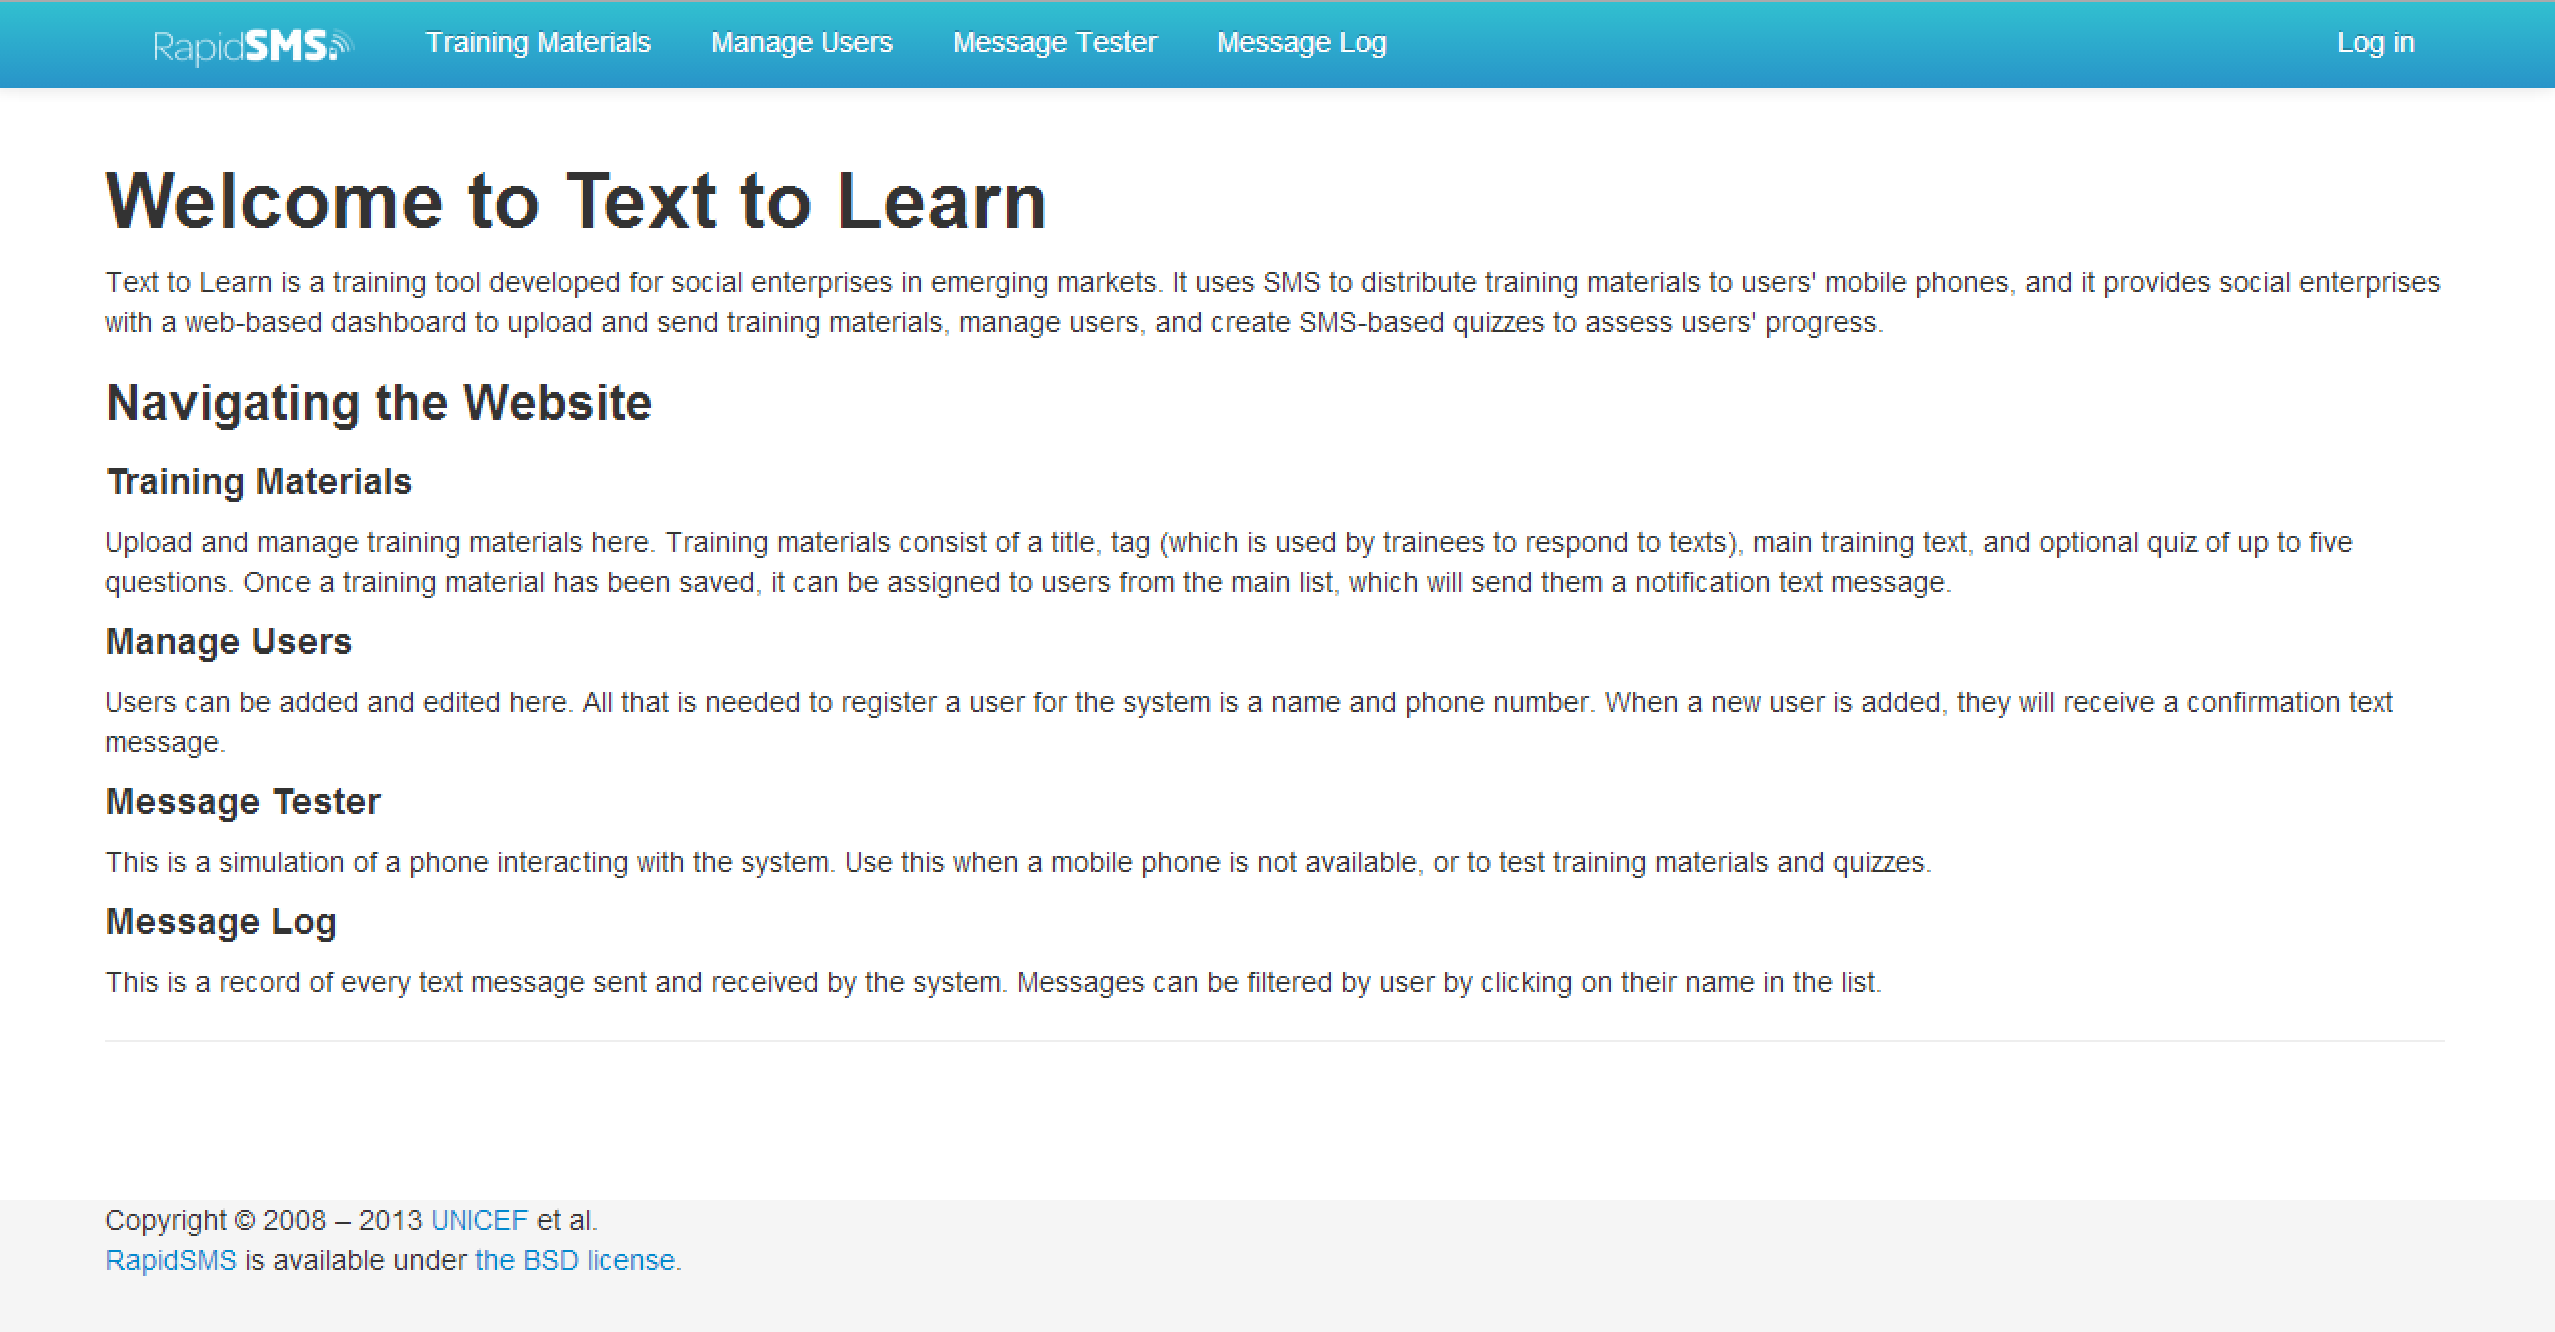
\includegraphics[scale=0.15]{home.png}
	\caption{Home page}
\end{figure}

\begin{figure}[H]
	\centering
	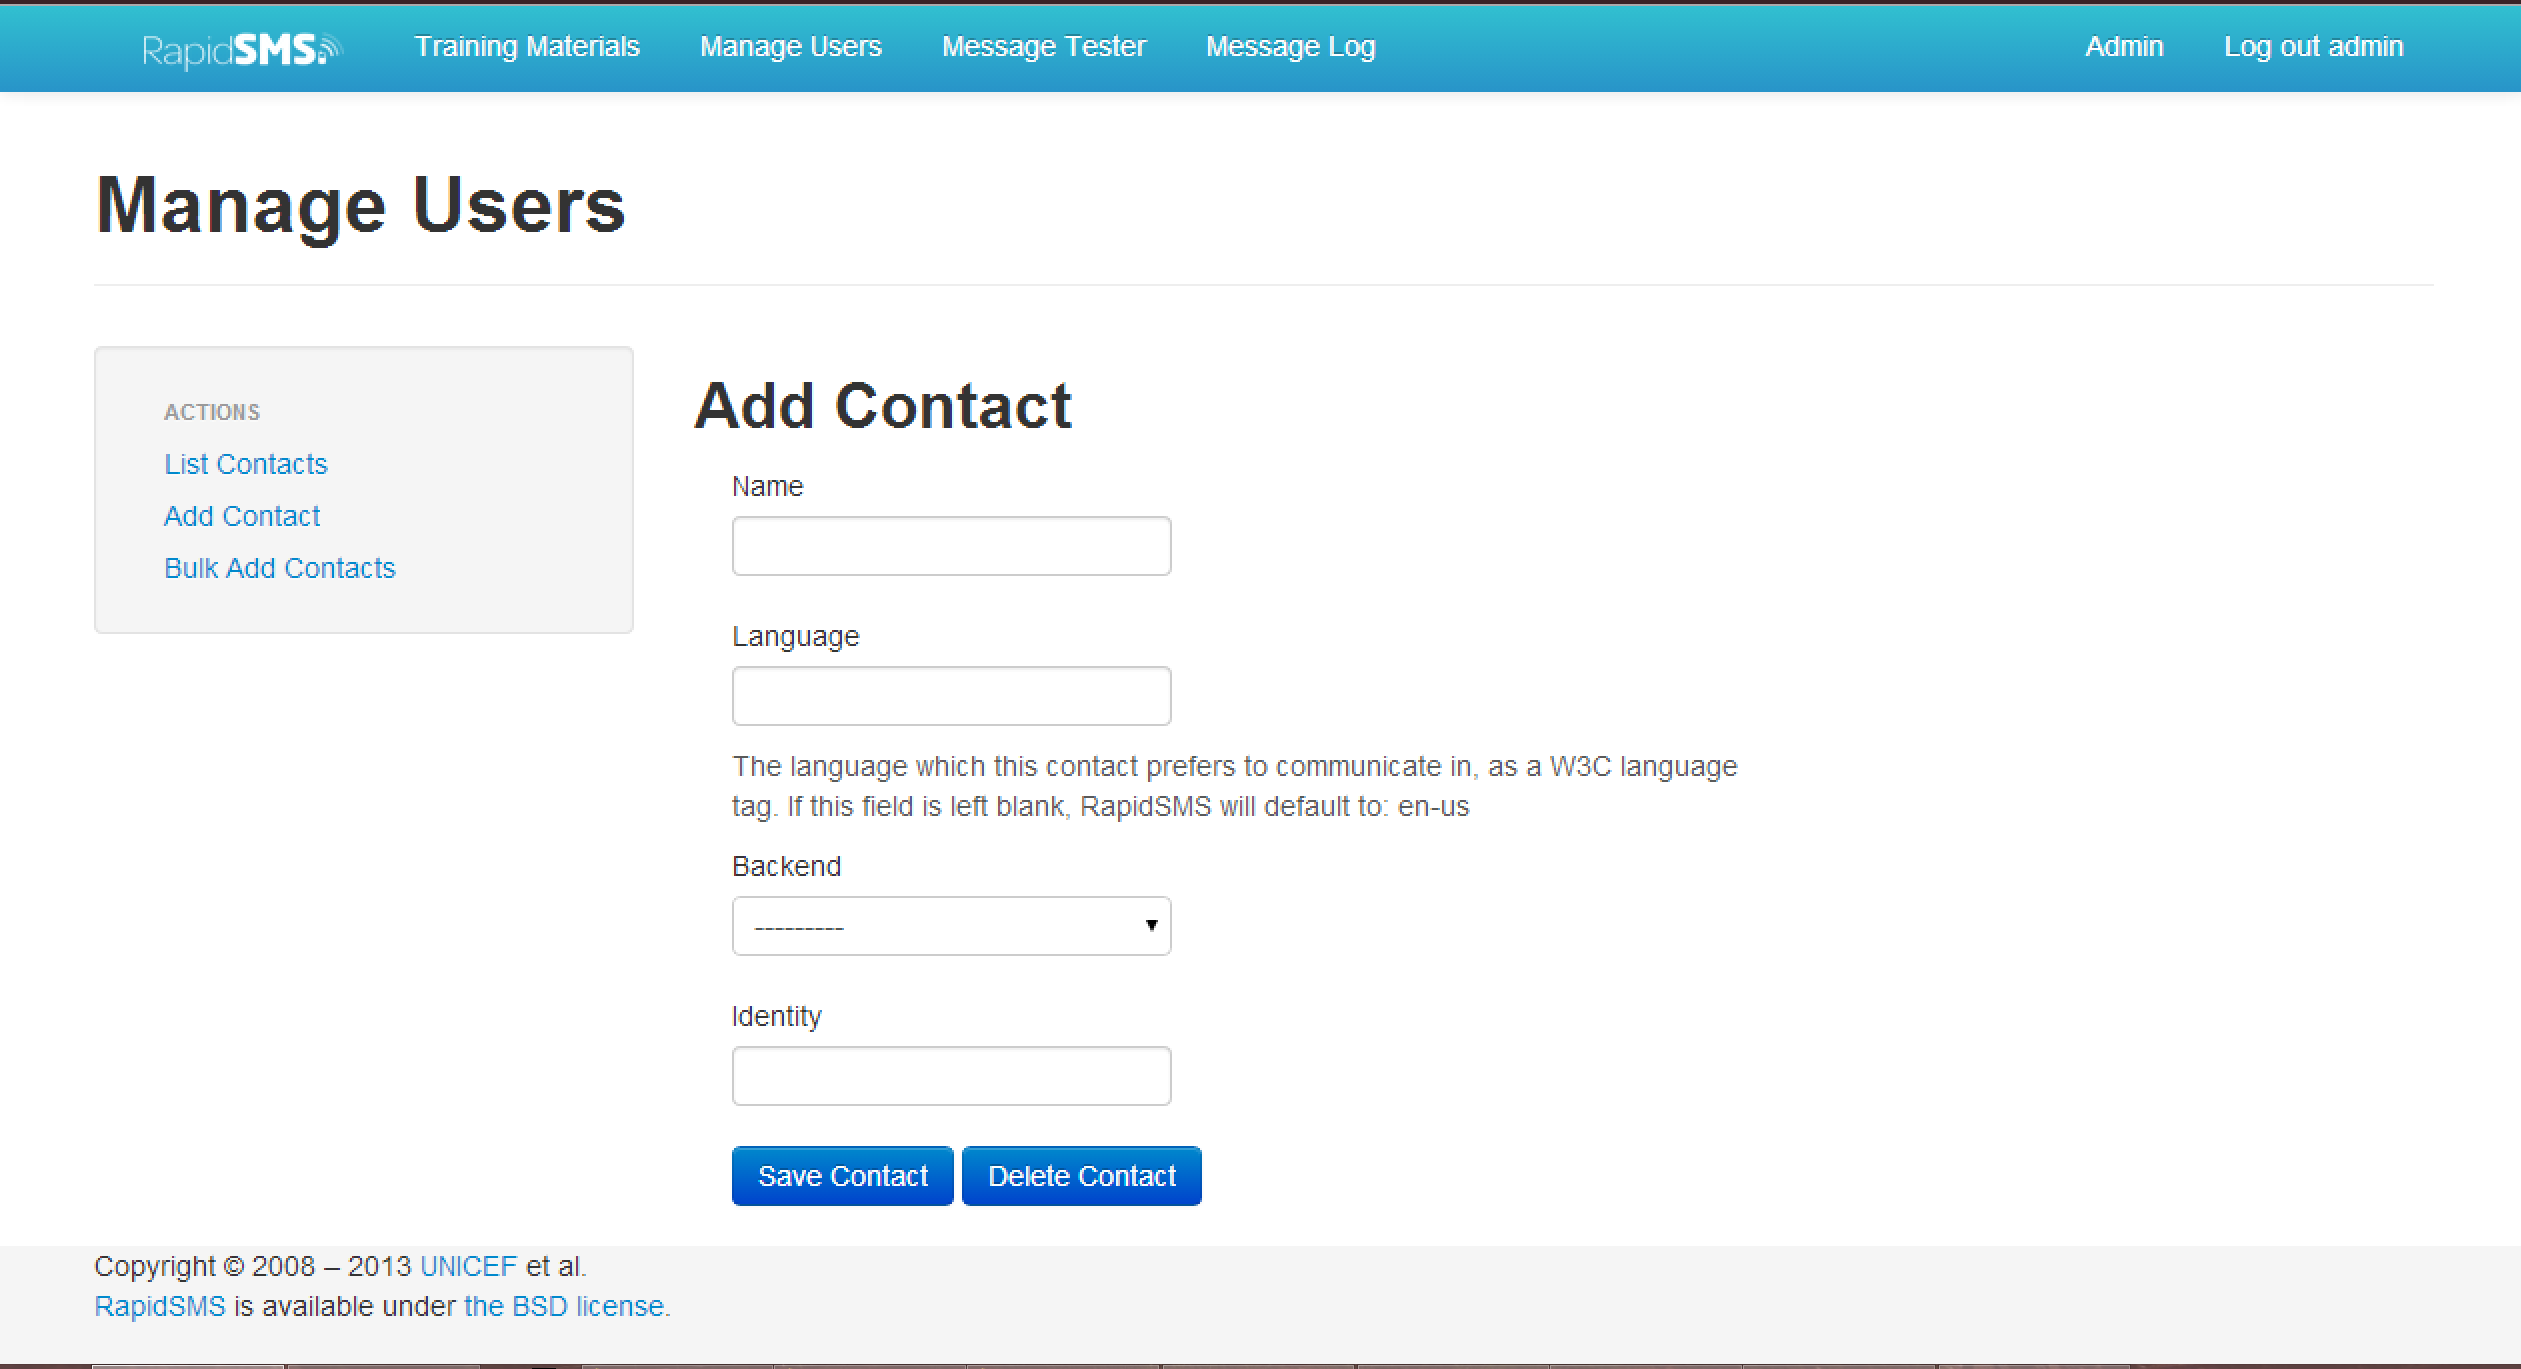
\includegraphics[scale=0.15]{add_contact.png}
	\caption{Add a User}
\end{figure}

\begin{figure}[H]
	\centering
	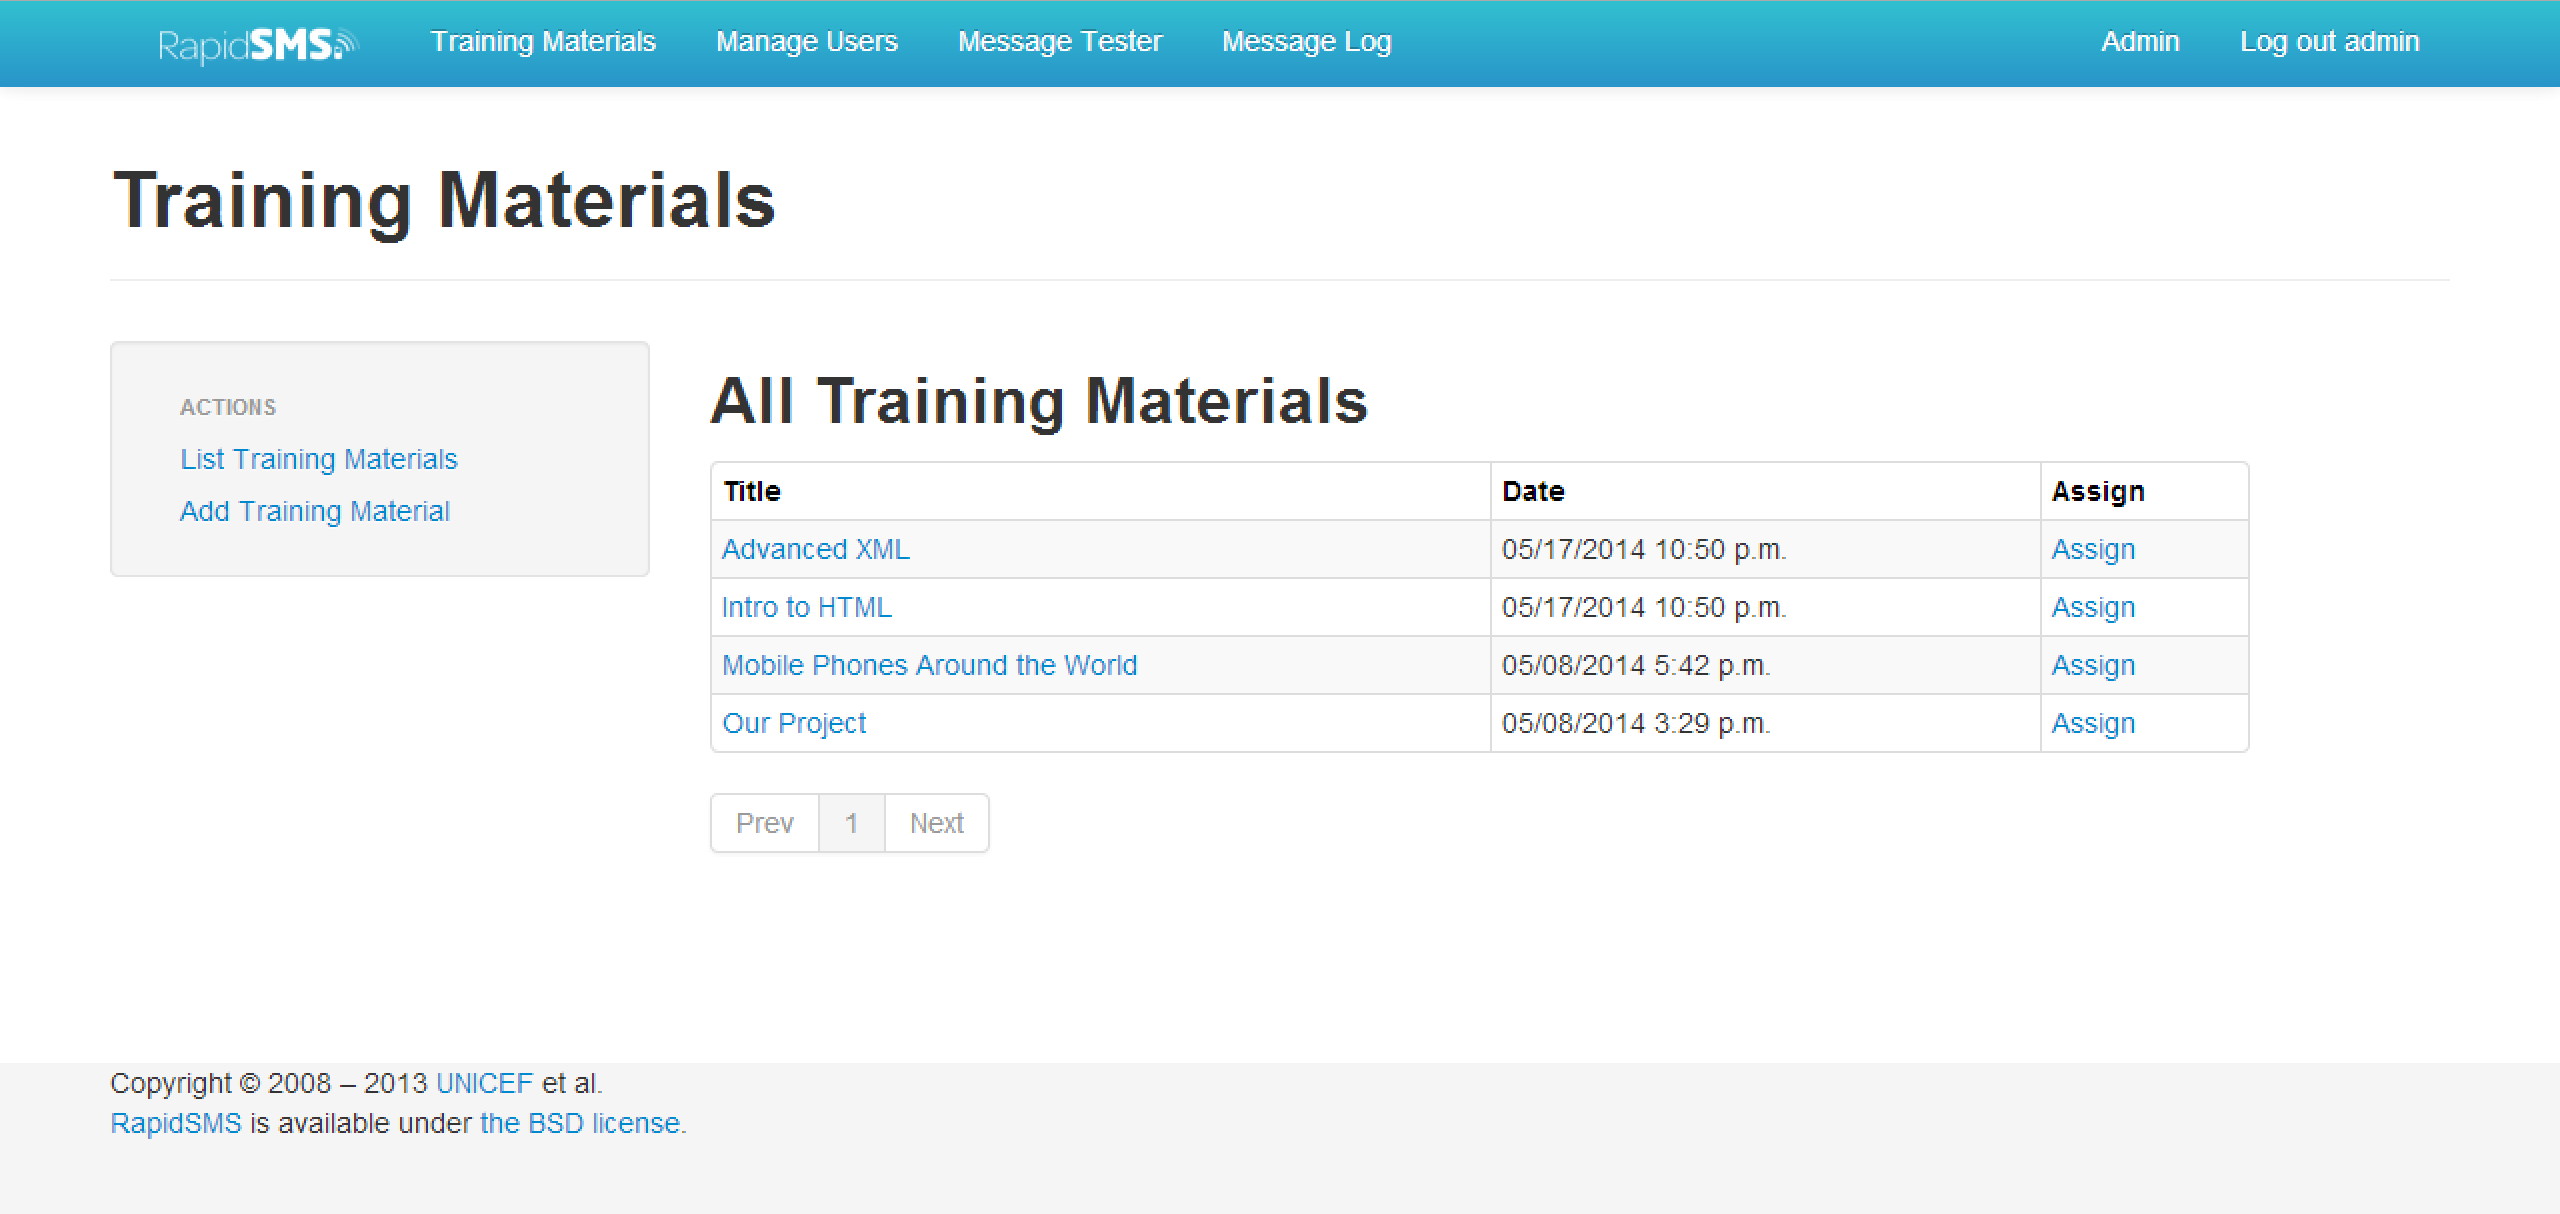
\includegraphics[scale=0.15]{list_tm.png}
	\caption{Training Materials}
\end{figure}

\begin{figure}[H]
	\centering
	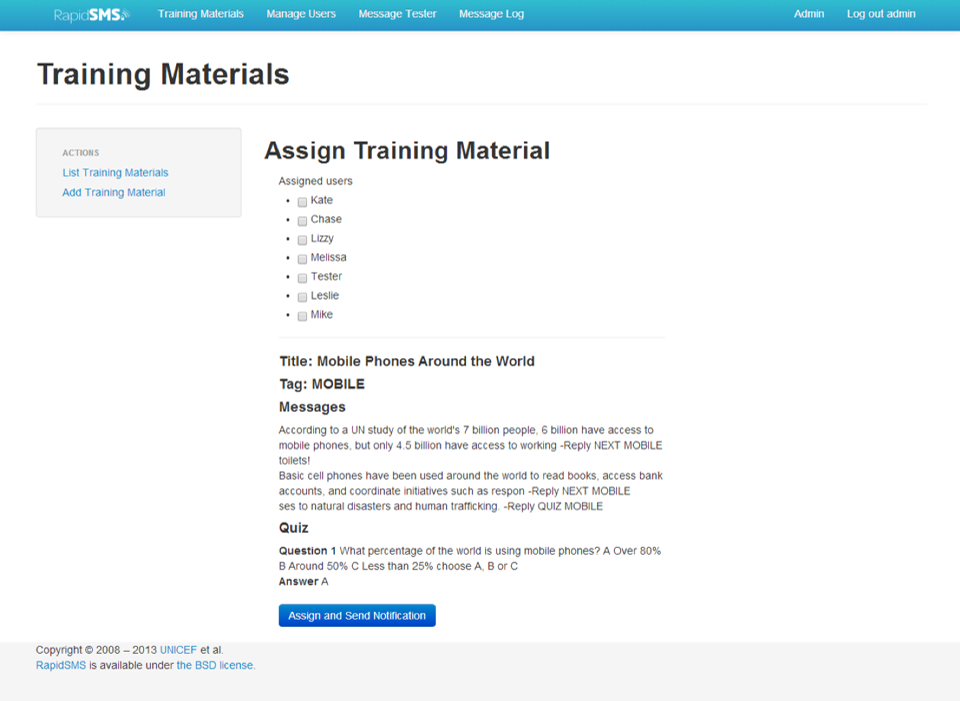
\includegraphics[scale=0.62]{assign_tm.png}
	\caption{Assign Training Material to Users}
\end{figure}

\begin{figure}[H]
	\centering
	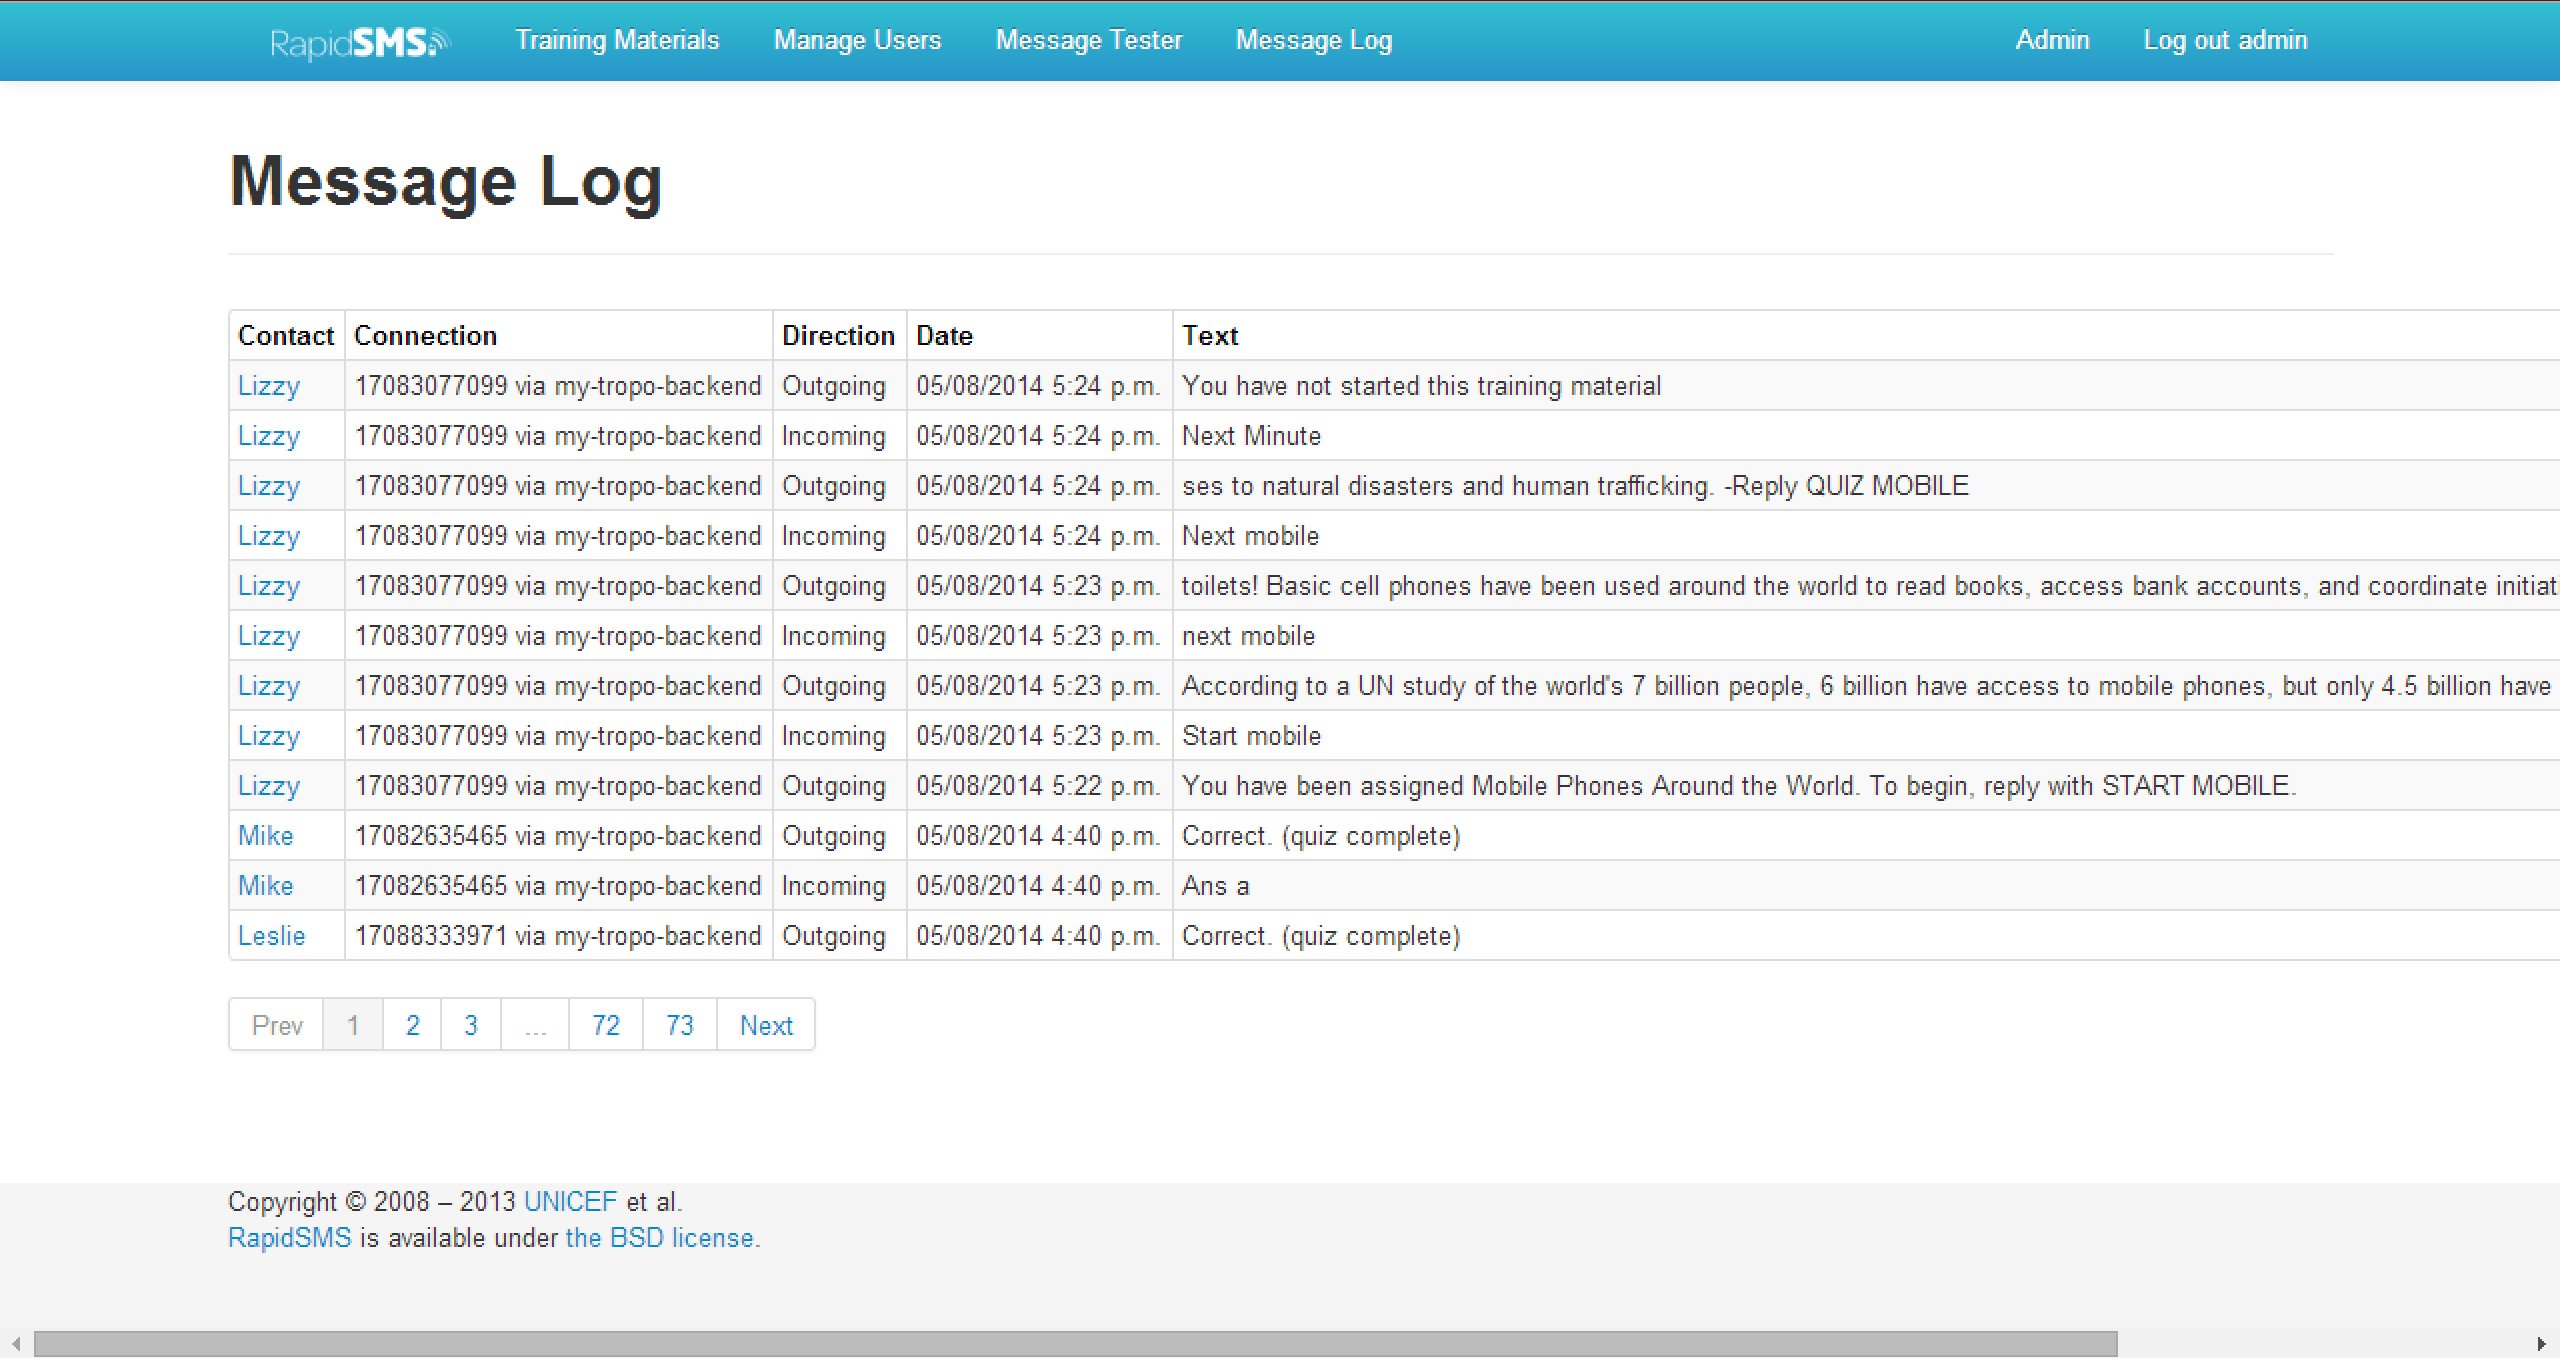
\includegraphics[scale=0.15]{message_log.png}
	\caption{Message Log}
\end{figure}


\section{Trainee Interaction: The Phone}
Trainees, or the users that are registered for Text to Learn, interact with the system through their mobile phones via SMS text messaging. Once their phone number has been registered by a trainer, they are able to text the Text to Learn phone number. At any time, a user can get help for using our system using the \textit{HELP} command.


\begin{table}[H]
    \begin{tabular}{ | 1 | 1 | 1 | p{5cm} |}
    \hline
    Status & Text Received by Trainee \\ \hline
    Once assigned a training material & You have been assigned <training material name>. To begin, reply with START <TM tag>.  \\ \hline
    After starting a training material & 9C  \\ \hline
    At final message of training material with a quiz & 10C \\ \hline
    At final message of training material witouth a quiz & 9C  \\ \hline
    At final message of quiz & 9C  \\ 
    \hline
    \caption{Table taken from}
    \end{tabular}
\end{table}
	

\section{System Design}
The following diagrams show our design visually by specifying the three main components of our system (webpage, cloud storage, and SMS service), the main functionality of each component, and how they interact with each other.

Our system is designed around three main components: a website, SMS, and cloud storage. The website is the way trainers or distributors interact with the system. Through the website, trainers can login to the office of their choosing and manage users, add new training materials and quizzes, and view, edit, and manage previously uploaded training materials and quizzes. To add users, the trainer simply needs to know the trainee's phone number and add it into the system. Adding new training materials and quizzes requires trainers to have these in plain text format and then copy and paste them into the appropriate text fields. From there, the materials can be assigned and sent to trainees via SMS. Through the website's message log, the trainers are able to view every message sent and received by the system, and filter this by user to see a particular user's responses to a quiz.

\begin{figure}[H]
	\centering
	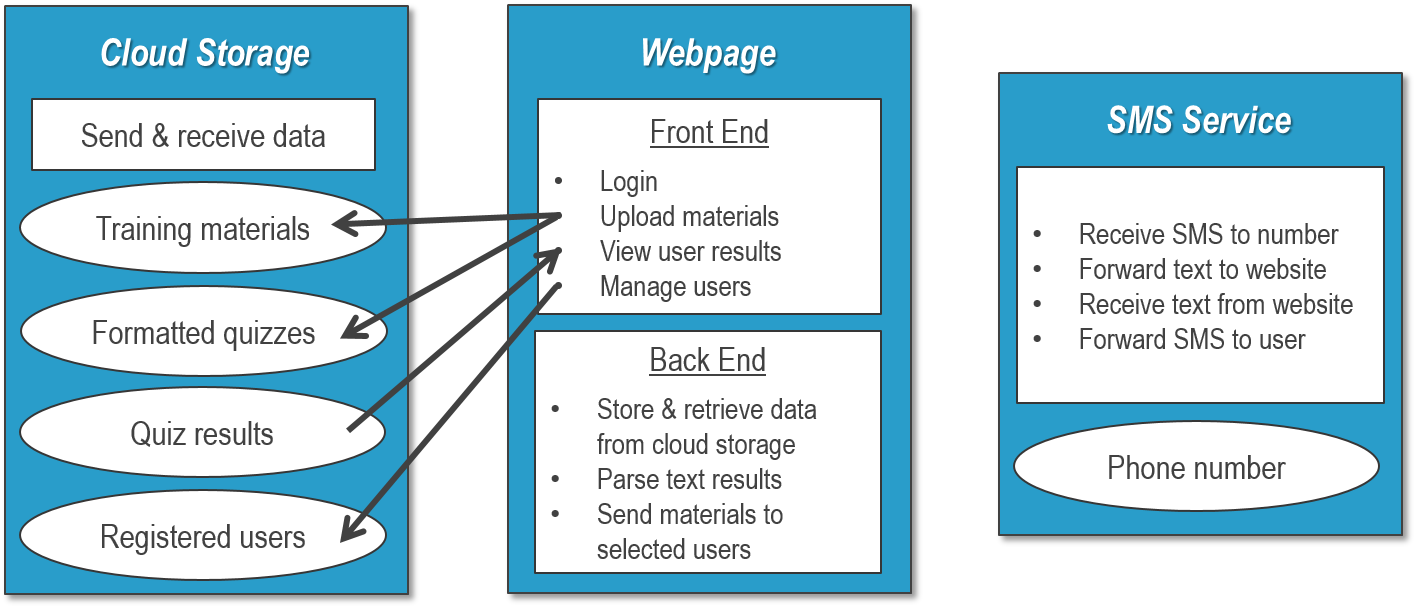
\includegraphics[scale=0.5]{trainer.png}
	\caption{System Diagram for Trainer}
\end{figure}

Trainees will interact with the system through SMS. ...

\begin{figure}[H]
	\centering
	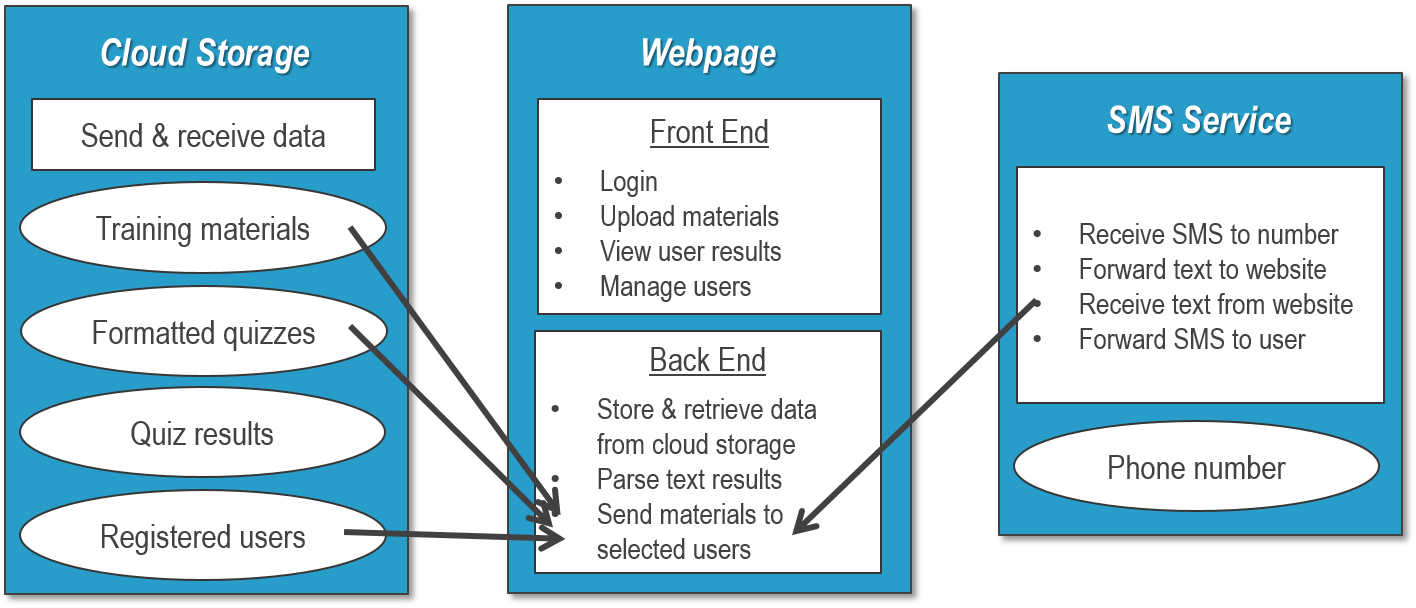
\includegraphics[scale=0.5]{trainee_request.png}
	\caption{System Diagram for Trainee Request}
\end{figure}

\begin{figure}[H]
	\centering
	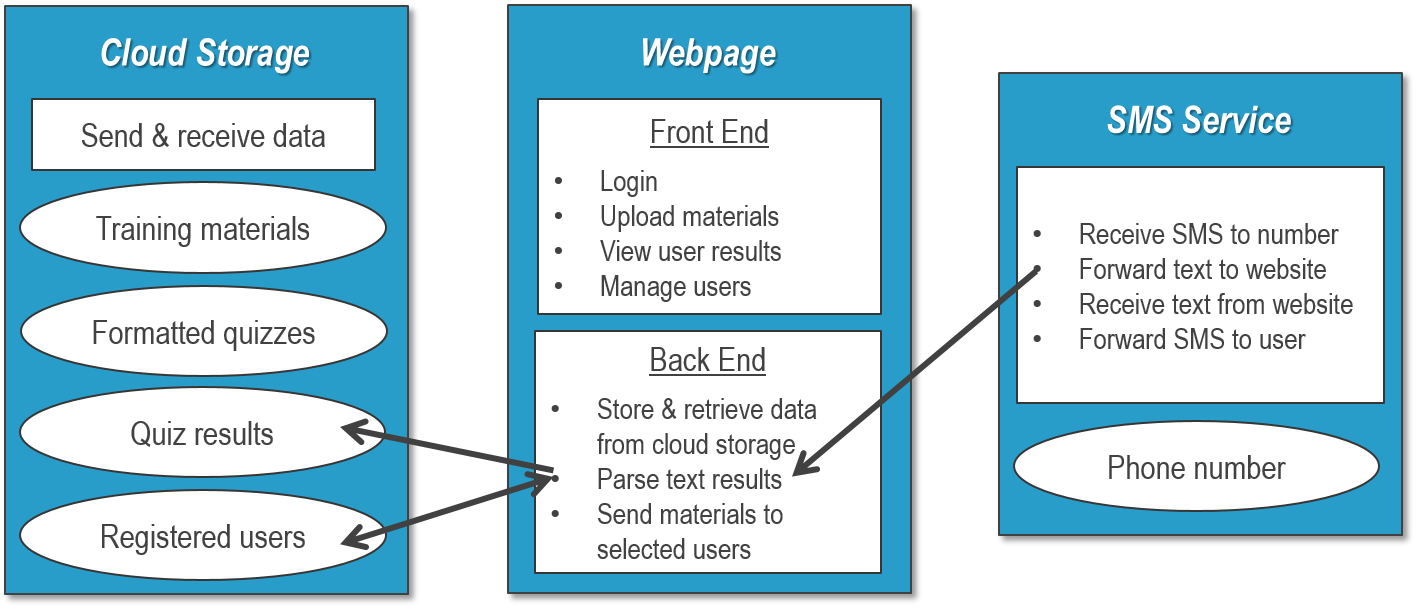
\includegraphics[scale=0.5]{trainee.png}
	\caption{System Diagram for Trainee}
\end{figure}

\section{Technologies Used}
\begin{description}
	\item[RapidSMS] a recent UNICEF project built to integrate SMS services with the Django web-framework
	\begin{description}
		\item[Django] a web-framework that lends itself to form collections
		\item[Python] the primary programming language used in Django
	\end{description}
	\item[dotCloud] a cloud web-hosting service that hosts our website in a Python web server and our data in a PostgreSQL database
	\item[Tropo] a web-based SMS service that generates a phone number and API to connect to websites
	\item[GitHub] version control system
\end{description}

\section{Design Rationale}

We chose to use a cloud service for storage rather than a local server. The cloud service holds all of the information that is sent and received between trainers and trainees, including training documents, formatted quizzes, quiz results, and registered users. Storing information “in the cloud” means that it can be accessed by other people directly through the internet, so trainers have access to this information from any computer with internet connection, whether at the office or at home. The cloud offers storage for large amounts of data, so trainers will not be limited by storage space when uploading training materials. The alternative to using cloud storage would be to have all of the training materials stored on a server belonging to the individual social enterprise. We decided against this option because cloud computing is the technology of the future. Although all social enterprises may not have the capability to use cloud services at their offices currently, cloud computing is growing rapidly in popularity and is sure to be utilized by more social enterprises eventually.

We considered building our system as a native phone apps, however we saw more barriers to this approach versus an SMS-based system. Since our target audience will often have the most basic phones, their phones may not be able to support even Java applications that are available on most feature phones, and would require use of the internet which again is often not supported. Even if these problems were not a barrier, the application would need to be installed on the phone, and not all phones have a way to install applications via the Web and may require the phone owner to go to their office to install the application. Essentially, using SMS has virtually no startup costs, and it will reach the broadest audience possible in emerging markets.

The system will also be using a paid SMS service to manage incoming and outgoing texts. While we could have written scripts to send texts from an email address for free, we would have needed to know the user’s service provider, and that service provider must have an email domain which may not be extensible to developing countries. There are open source models that work by plugging a gsm modem with a sim card into a computer to receive texts, but these are often difficult to work with and hard to scale. For these reasons, we made the decision to use a paid SMS service rather than using an email address to handle text messaging.

\chapter{Testing and Documentation}

\section{Testing}

\section{Documentation}
\chapter{Project Management}

\section{Project Schedule}
Our development timeline for completing various portions of the project is defined in the Gantt charts (see \textbf{Appendix A}). There is one chart per quarter, with the fall quarter chart displaying the actual weekly timeline for the work we have already accomplished, and the winter and spring quarter charts displaying the intended weekly timeline for the work we will accomplish in the future.

\section{Risk Management}
In addition to creating a schedule of when to complete different tasks for our project, we have also compiled a list of potential risks to our project, including their probability of occurring, severity, and total impact. We have also included mitigation strategies for each risk so that if a risk does occur, we will be prepared for it. These are defined in the following risk analysis chart, Table 1:
\chapter{Societal Issues}
\chapter{Conclusions}

\section{Summary}

\section{Lessons Learned}

\section{Future Improvements}


\backmatter
\pagenumbering{Roman}
\chapter{Appendices}

\section{Project Schedule}
\begin{figure}[H]
	\centering
	
\includegraphics[scale=0.7]{schedule_fall.png}
	\caption{Gantt Chart for Fall Quarter}
\end{figure}

\begin{figure}[H]
	\centering
	
\includegraphics[scale=0.7]{schedule_winter.png}
	\caption{Gantt Chart for Winter Quarter}
\end{figure}

\begin{figure}[H]
	\centering
	
\includegraphics[scale=0.7]{schedule_fall.png}
	\caption{Gantt Chart for Spring Quarter}
\end{figure}

\begin{table}[H]
	\centering
	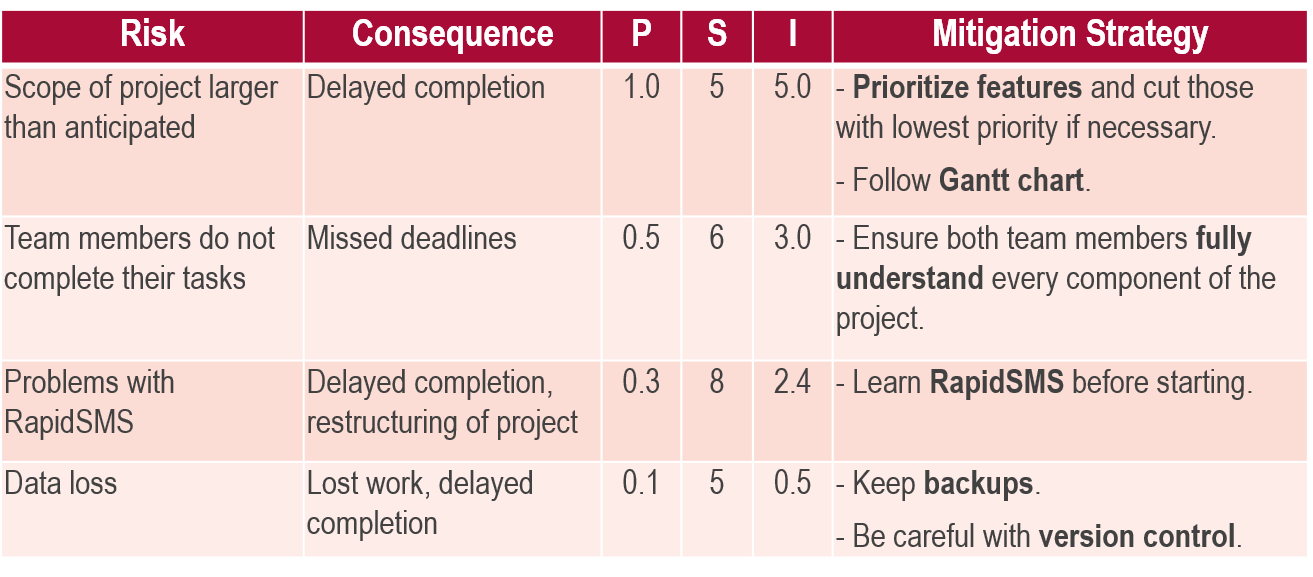
\includegraphics[scale=0.7]{risks.png}
	\caption{Risk Analysis}
\end{table}


\section{Setup and Installation}
This project is currently configured to be hosted on dotCloud with a Python server and PostgreSQL database and connects to a Tropo SMS backend. This manual will detail how to switch to your own subscription of dotCloud and Tropo and what to delete if you wish to replace Tropo with your own service.

\subsection*{General}
You will need Python on your system, Python 2.7 is recommended. https://www.python.org/download/releases/2.7
You will also ideally be using something unix based (Mac or Linux) if you are on a Windows machine try using Cygwin, but this has had mixed results.

\subsection*{Using your own dotCloud Credentials}
In order to deploy to dotCloud you will need to have python already installed on your computer. The code for this project was gotten from this github project, please see their documentation if you need additional instructions: https://github.com/caktus/rapidsms-deploy-dotcloud

Once you have Python 2.7 installed navigate to that folder through the terminal (or Cygwin) and follow the instructions in dotCloud installation instructions. http://docs.dotcloud.com/firststeps/install/
This will ask for your personal credentials, no changes to the code should be necessary.

You should now be able to push using “dotcloud push” in the terminal. This process may take some time

For adding custom domains see the following dotCloud documentation: http://docs.dotcloud.com/guides/domains/

\subsection*{Using your own Tropo backend}
You will need to modify code. You will need to get your account authorized before you can send outgoing messages. For help setting up your Tropo account  or trouble shooting the installation see this rapidSMS tutorial: http://rapidsms.readthedocs.org/en/latest/tutorial/tutorial04.html\#tutorial04

To complete this next part have your outgoing messaging token and Tropo phone number ready. 

\begin{enumerate}
	\item In the rapidsms\_tut folder open the settings.py file
	\item At nearly the bottom of the file, look for "INSTALLED\_BACKENDS = " in this section you should find 
	\begin{verbatim}
	    "my-tropo-backend": {
	        "ENGINE": "rtropo.outgoing.TropoBackend",
	        'config': {
	            'messaging\_token': '[insert_token]',
	            'number': '[+1-555-555-5555']’,
	        },
	    },
	\end{verbatim}
	\item Change the string under ‘messaging token’ to your messaging token
	\item Change the ‘number’ to you number, make sure you start with a ‘+’ followed by your country code
\end{enumerate}

\subsection*{Removing Tropo}
WARNING: Following these steps after you have created contacts with “my-tropo-backend” may result in critical errors. Be sure to delete any contacts with this backend first.

You will need to edit three files rapidsms\_tut/settings.py, rapidsms\_tut/urls.py, and requirements/base.py.

settings.py
\begin{enumerate}
	\item As in the previous section open settings.py in the rapidsms\_tut folder
	\item Delete the lines of code show in step 2 of the previous section

\subsubsection*{urls.py}
 	\item Open urls.py (also in the rapidsms\_tut folder)
	\item Delete the following lines of code:
    url(r'\^tropo/',
      message\_received,
      kwargs={'backend\_name': 'my-tropo-backend'}),
\subsubsection*{base.py}
	\item From the main folder navigate to the ‘requirements’ folder and open base.txt
	\item Delete the line rapidsms-tropo>=0.2.0

	\item After saving all these files, you should be able to “dotcloud push” and “my-tropo-backend” will no longer be available.
\end{enumerate}



\section{User Manual}

\section{Source Code}

\end{document}
